\begin{figure}[H]
    \centering
    \begin{subfigure}{0.4\textwidth}
        \centering
        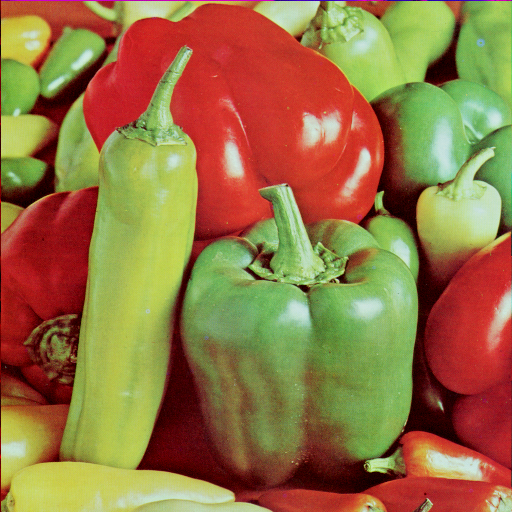
\includegraphics[width=0.85\textwidth]{pep_perm/imagem.png}
        \caption{Imagem com mensagem oculta.}
        \label{fig:permtexto:imagem}
    \end{subfigure}%
    \begin{subfigure}{0.4\textwidth}
        \centering
        \includegraphics[width=0.85\textwidth]{pep_perm/plano0.png}
        \caption{Plano 0.}
        \label{fig:permtexto:plano}
    \end{subfigure}\\[8pt]
    \begin{subfigure}{0.28\textwidth}
        \centering
        \includegraphics[width=0.85\textwidth]{pep_perm/pl0chb.png}
        \caption{Plano 0, canal azul.}
        \label{fig:permtexto:blue}
    \end{subfigure}%
    \begin{subfigure}{0.28\textwidth}
        \centering
        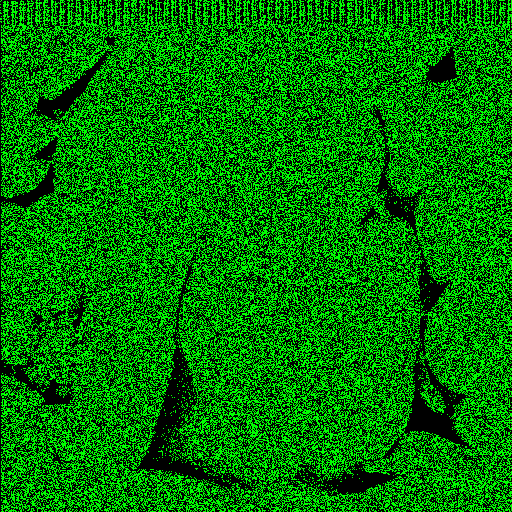
\includegraphics[width=0.85\textwidth]{pep_perm/pl0chg.png}
        \caption{Plano 0, canal verde.}
        \label{fig:permtexto:green}
    \end{subfigure}%
    \begin{subfigure}{0.28\textwidth}
        \centering
        \includegraphics[width=0.85\textwidth]{pep_perm/pl0chr.png}
        \caption{Plano 0, canal vermelho.}
        \label{fig:permtexto:red}
    \end{subfigure}%

    \caption{\cref{fig:pequeno} com permutação dos dados.}
    \label{fig:permtexto}
\end{figure}